% Options for packages loaded elsewhere
\PassOptionsToPackage{unicode}{hyperref}
\PassOptionsToPackage{hyphens}{url}
\PassOptionsToPackage{dvipsnames,svgnames,x11names}{xcolor}
%
\documentclass[
  letterpaper,
  DIV=11,
  numbers=noendperiod]{scrartcl}

\usepackage{amsmath,amssymb}
\usepackage{lmodern}
\usepackage{iftex}
\ifPDFTeX
  \usepackage[T1]{fontenc}
  \usepackage[utf8]{inputenc}
  \usepackage{textcomp} % provide euro and other symbols
\else % if luatex or xetex
  \usepackage{unicode-math}
  \defaultfontfeatures{Scale=MatchLowercase}
  \defaultfontfeatures[\rmfamily]{Ligatures=TeX,Scale=1}
\fi
% Use upquote if available, for straight quotes in verbatim environments
\IfFileExists{upquote.sty}{\usepackage{upquote}}{}
\IfFileExists{microtype.sty}{% use microtype if available
  \usepackage[]{microtype}
  \UseMicrotypeSet[protrusion]{basicmath} % disable protrusion for tt fonts
}{}
\makeatletter
\@ifundefined{KOMAClassName}{% if non-KOMA class
  \IfFileExists{parskip.sty}{%
    \usepackage{parskip}
  }{% else
    \setlength{\parindent}{0pt}
    \setlength{\parskip}{6pt plus 2pt minus 1pt}}
}{% if KOMA class
  \KOMAoptions{parskip=half}}
\makeatother
\usepackage{xcolor}
\setlength{\emergencystretch}{3em} % prevent overfull lines
\setcounter{secnumdepth}{-\maxdimen} % remove section numbering
% Make \paragraph and \subparagraph free-standing
\ifx\paragraph\undefined\else
  \let\oldparagraph\paragraph
  \renewcommand{\paragraph}[1]{\oldparagraph{#1}\mbox{}}
\fi
\ifx\subparagraph\undefined\else
  \let\oldsubparagraph\subparagraph
  \renewcommand{\subparagraph}[1]{\oldsubparagraph{#1}\mbox{}}
\fi

\usepackage{color}
\usepackage{fancyvrb}
\newcommand{\VerbBar}{|}
\newcommand{\VERB}{\Verb[commandchars=\\\{\}]}
\DefineVerbatimEnvironment{Highlighting}{Verbatim}{commandchars=\\\{\}}
% Add ',fontsize=\small' for more characters per line
\usepackage{framed}
\definecolor{shadecolor}{RGB}{241,243,245}
\newenvironment{Shaded}{\begin{snugshade}}{\end{snugshade}}
\newcommand{\AlertTok}[1]{\textcolor[rgb]{0.68,0.00,0.00}{#1}}
\newcommand{\AnnotationTok}[1]{\textcolor[rgb]{0.37,0.37,0.37}{#1}}
\newcommand{\AttributeTok}[1]{\textcolor[rgb]{0.40,0.45,0.13}{#1}}
\newcommand{\BaseNTok}[1]{\textcolor[rgb]{0.68,0.00,0.00}{#1}}
\newcommand{\BuiltInTok}[1]{\textcolor[rgb]{0.00,0.23,0.31}{#1}}
\newcommand{\CharTok}[1]{\textcolor[rgb]{0.13,0.47,0.30}{#1}}
\newcommand{\CommentTok}[1]{\textcolor[rgb]{0.37,0.37,0.37}{#1}}
\newcommand{\CommentVarTok}[1]{\textcolor[rgb]{0.37,0.37,0.37}{\textit{#1}}}
\newcommand{\ConstantTok}[1]{\textcolor[rgb]{0.56,0.35,0.01}{#1}}
\newcommand{\ControlFlowTok}[1]{\textcolor[rgb]{0.00,0.23,0.31}{#1}}
\newcommand{\DataTypeTok}[1]{\textcolor[rgb]{0.68,0.00,0.00}{#1}}
\newcommand{\DecValTok}[1]{\textcolor[rgb]{0.68,0.00,0.00}{#1}}
\newcommand{\DocumentationTok}[1]{\textcolor[rgb]{0.37,0.37,0.37}{\textit{#1}}}
\newcommand{\ErrorTok}[1]{\textcolor[rgb]{0.68,0.00,0.00}{#1}}
\newcommand{\ExtensionTok}[1]{\textcolor[rgb]{0.00,0.23,0.31}{#1}}
\newcommand{\FloatTok}[1]{\textcolor[rgb]{0.68,0.00,0.00}{#1}}
\newcommand{\FunctionTok}[1]{\textcolor[rgb]{0.28,0.35,0.67}{#1}}
\newcommand{\ImportTok}[1]{\textcolor[rgb]{0.00,0.46,0.62}{#1}}
\newcommand{\InformationTok}[1]{\textcolor[rgb]{0.37,0.37,0.37}{#1}}
\newcommand{\KeywordTok}[1]{\textcolor[rgb]{0.00,0.23,0.31}{#1}}
\newcommand{\NormalTok}[1]{\textcolor[rgb]{0.00,0.23,0.31}{#1}}
\newcommand{\OperatorTok}[1]{\textcolor[rgb]{0.37,0.37,0.37}{#1}}
\newcommand{\OtherTok}[1]{\textcolor[rgb]{0.00,0.23,0.31}{#1}}
\newcommand{\PreprocessorTok}[1]{\textcolor[rgb]{0.68,0.00,0.00}{#1}}
\newcommand{\RegionMarkerTok}[1]{\textcolor[rgb]{0.00,0.23,0.31}{#1}}
\newcommand{\SpecialCharTok}[1]{\textcolor[rgb]{0.37,0.37,0.37}{#1}}
\newcommand{\SpecialStringTok}[1]{\textcolor[rgb]{0.13,0.47,0.30}{#1}}
\newcommand{\StringTok}[1]{\textcolor[rgb]{0.13,0.47,0.30}{#1}}
\newcommand{\VariableTok}[1]{\textcolor[rgb]{0.07,0.07,0.07}{#1}}
\newcommand{\VerbatimStringTok}[1]{\textcolor[rgb]{0.13,0.47,0.30}{#1}}
\newcommand{\WarningTok}[1]{\textcolor[rgb]{0.37,0.37,0.37}{\textit{#1}}}

\providecommand{\tightlist}{%
  \setlength{\itemsep}{0pt}\setlength{\parskip}{0pt}}\usepackage{longtable,booktabs,array}
\usepackage{calc} % for calculating minipage widths
% Correct order of tables after \paragraph or \subparagraph
\usepackage{etoolbox}
\makeatletter
\patchcmd\longtable{\par}{\if@noskipsec\mbox{}\fi\par}{}{}
\makeatother
% Allow footnotes in longtable head/foot
\IfFileExists{footnotehyper.sty}{\usepackage{footnotehyper}}{\usepackage{footnote}}
\makesavenoteenv{longtable}
\usepackage{graphicx}
\makeatletter
\def\maxwidth{\ifdim\Gin@nat@width>\linewidth\linewidth\else\Gin@nat@width\fi}
\def\maxheight{\ifdim\Gin@nat@height>\textheight\textheight\else\Gin@nat@height\fi}
\makeatother
% Scale images if necessary, so that they will not overflow the page
% margins by default, and it is still possible to overwrite the defaults
% using explicit options in \includegraphics[width, height, ...]{}
\setkeys{Gin}{width=\maxwidth,height=\maxheight,keepaspectratio}
% Set default figure placement to htbp
\makeatletter
\def\fps@figure{htbp}
\makeatother

\KOMAoption{captions}{tableheading}
\makeatletter
\makeatother
\makeatletter
\makeatother
\makeatletter
\@ifpackageloaded{caption}{}{\usepackage{caption}}
\AtBeginDocument{%
\ifdefined\contentsname
  \renewcommand*\contentsname{Table of contents}
\else
  \newcommand\contentsname{Table of contents}
\fi
\ifdefined\listfigurename
  \renewcommand*\listfigurename{List of Figures}
\else
  \newcommand\listfigurename{List of Figures}
\fi
\ifdefined\listtablename
  \renewcommand*\listtablename{List of Tables}
\else
  \newcommand\listtablename{List of Tables}
\fi
\ifdefined\figurename
  \renewcommand*\figurename{Figure}
\else
  \newcommand\figurename{Figure}
\fi
\ifdefined\tablename
  \renewcommand*\tablename{Table}
\else
  \newcommand\tablename{Table}
\fi
}
\@ifpackageloaded{float}{}{\usepackage{float}}
\floatstyle{ruled}
\@ifundefined{c@chapter}{\newfloat{codelisting}{h}{lop}}{\newfloat{codelisting}{h}{lop}[chapter]}
\floatname{codelisting}{Listing}
\newcommand*\listoflistings{\listof{codelisting}{List of Listings}}
\makeatother
\makeatletter
\@ifpackageloaded{caption}{}{\usepackage{caption}}
\@ifpackageloaded{subcaption}{}{\usepackage{subcaption}}
\makeatother
\makeatletter
\@ifpackageloaded{tcolorbox}{}{\usepackage[many]{tcolorbox}}
\makeatother
\makeatletter
\@ifundefined{shadecolor}{\definecolor{shadecolor}{rgb}{.97, .97, .97}}
\makeatother
\makeatletter
\makeatother
\ifLuaTeX
  \usepackage{selnolig}  % disable illegal ligatures
\fi
\IfFileExists{bookmark.sty}{\usepackage{bookmark}}{\usepackage{hyperref}}
\IfFileExists{xurl.sty}{\usepackage{xurl}}{} % add URL line breaks if available
\urlstyle{same} % disable monospaced font for URLs
\hypersetup{
  pdftitle={Why R?},
  pdfauthor={Harshvardhan},
  colorlinks=true,
  linkcolor={blue},
  filecolor={Maroon},
  citecolor={Blue},
  urlcolor={Blue},
  pdfcreator={LaTeX via pandoc}}

\title{Why R?}
\usepackage{etoolbox}
\makeatletter
\providecommand{\subtitle}[1]{% add subtitle to \maketitle
  \apptocmd{\@title}{\par {\large #1 \par}}{}{}
}
\makeatother
\subtitle{A Brief Introduction to My Favourite Language}
\author{Harshvardhan}
\date{}

\begin{document}
\maketitle
\ifdefined\Shaded\renewenvironment{Shaded}{\begin{tcolorbox}[frame hidden, borderline west={3pt}{0pt}{shadecolor}, interior hidden, sharp corners, boxrule=0pt, breakable, enhanced]}{\end{tcolorbox}}\fi

\begin{quote}
\emph{There are only two kinds of languages: the ones people complain
about and the ones nobody uses.}

--- Bjarne Stroustrup
\end{quote}

\hypertarget{what-is-r}{%
\section{What is R?}\label{what-is-r}}

Roger Peng called R Programming Language a dialect of S
language.\footnote{Peng, Roger D. \emph{R programming for data science}.
  Victoria, BC, Canada: Leanpub, 2016.} Though I would say this dialect
deserves a place among the ``important'' languages as its own, it begs
the question: what is S? S is a programming language developed as an
internal statistical analysis tool at AT\&T Bell Laboratories. It was
initiated in 1976 when computer programs were not commonplace for
statistical analyses. The Bell Labs scientists would go to talks and
show amazing graphics and results --- sometimes even live demos.

Soon, statisticians everywhere wanted to use it for their analyses. Bell
Labs was conservative in sharing the software with the broader public;
it was an internal tool. Even if it was made available, there were
several roadblocks. First, you needed a Unix computer to run S. You
would need a modem connecting to the Bell Labs and using their computing
powers. Second, there was no binary installation file like ``.exe'' or
``.dmg'' that you could double-click and go. You would get the source
code from Bell Labs, and you had to compile it yourself.

Let's say you were brave enough to attempt compiling it yourself. But in
those days, processors were not standardized.\footnote{Even today, when
  Apple launched M1, it took a lot of time for the developers to create
  native programs for Apple's M1 chip. M1 and M2 Macs have Rosetta 2,
  which could convert Intel-based software to a format required by M1.}
Every processor has different requirements. In 1993, Bell Labs gave an
exclusive license to StatSci (which later became Insightful Corp.) to
develop and sell S. Insightful added some bells and whistles to it and
made it S-Plus. S-Plus quickly gained popularity. It was available as a
binary installation file for Unix and Microsoft Windows.

In the first half of the 1990s, Ross Ihaka and Robert Gentleman, two
professors in the Department of Statistics at the University of
Auckland, wondered if a Macintosh version was available. The department
had recently gotten many of Apple's latest computers and needed software
for their statistics class. Since there was no S or S-Plus version for
Mac, they decided to write a version of the S language. Their first
attempt is noted in the classic paper published in the Journal of
Computational and Graphical Statistics.

\begin{quote}
Ross Ihaka and Robert Gentleman. R: A language for data analysis and
graphics. Journal of Computational and Graphical Statistics,
5(3):299--314, 1996
\end{quote}

Martin Mächler convinced them to release R with GNU General Public
License. This was critical for two reasons. First, it made R freely
available. Both S-Plus and S required a paid license. Second, it allowed
virtually anyone to tinker with its source code and suggest
improvements. Soon after, a mailing list was created where people shared
new enhancements. In 1997, R Core Group was formed, which, even today,
controls the source code of R. In 2000, R 1.0.0 was released to the
public.

Rest is history.

\hypertarget{what-can-r-do}{%
\section{What can R do?}\label{what-can-r-do}}

For this question, I asked \href{https://swatisonal.owlstown.net/}{Dr
Swati Sonal}, a postdoctoral research fellow at the Massachusetts
General Hospital and Harvard Medical School. She uses R for her
quantitative analyses, primarily focussed on clinical and translational
research in Colorectal Cancer. Here is what she had to say.

\begin{quote}
I think the primary reason I love R is that it is so cool! It makes me
feel like I'm analyzing without getting bogged down by the minute
programmatic details like one does in Python. I can do the ``default''
analysis, but it is simple to customize as per my requirements, which is
difficult to achieve in alternatives like SPSS and STATA. The output is
neat. I can get publication-ready tables and visualizations quickly.
There is nothing like the \textbf{dfSummary()} function, which can do
much so quickly.\footnote{\textbf{dfSummary()} is a function from the
  summaryTools package that can summarise data with a single command.
  Learn more:
  https://cran.r-project.org/web/packages/summarytools/vignettes/introduction.html}

Even making custom changes in them is intuitive. Functions are versatile
as well. No matter which model I use, I can always rely on
\textbf{predict()} for making predictions. R Markdown is handy for
reproducible research. Like a lab note, I can write my thoughts, do the
analysis and produce the results --- all using a single document.
Doesn't it sound like magic?
\end{quote}

\hypertarget{packages-and-cran}{%
\subsection{Packages and CRAN}\label{packages-and-cran}}

It is clear R can achieve a lot of things for free. Much of R's
functionalities are extended with packages, which are pieces of code
freely available for everyone to use.
\href{https://cran.r-project.org/index.html}{Comprehensive R Archive
Network (CRAN)} hosts the binary file for R software as well as an
archive of packages. The R software comes with specific default
capabilities, identified as ``base R''. Beyond that, it can be extended
by packages which one can install from
\href{https://cran.r-project.org/web/packages/available_packages_by_name.html}{CRAN},
GitHub, \href{https://www.bioconductor.org/}{Bioconductor}, among
others. \href{https://rdrr.io/}{rdrr.io} is an excellent search engine
for anything related to R, including R packages. On November 15, 2022,
it had information about 23,097 CRAN packages, 2,130 Bioconductor
packages, 2,207 R-Forge packages and 85,750 GitHub packages.

\hypertarget{rstudio}{%
\subsection{RStudio}\label{rstudio}}

RStudio is the most popular Integrated Development Environment (IDE) for
using R. The IDE provides a functional and beautiful interface to R with
a set of tools to help you be more productive with R. It has a built-in
console, Terminal, GitHub client, plot viewer, debugging tool, and a
host of other valuable appliances. I'd recommend you install R and
RStudio to get started with your R journey. Posit provides a
\href{https://posit.co/download/rstudio-desktop/}{simple guide} to do it
all.

Many custom functions can be added using add-ins. Dean Attali provides a
list of valuable add-ins in RStudio at
\url{https://github.com/daattali/addinslist}. Some of my favourite
add-ins are \href{https://github.com/dreamRs/esquisse}{esquisse}, which
offers a graphical interface for creating visualizations with ggplot2;
\href{https://github.com/MilesMcBain/datapasta}{datapasta}, with which
you can copy any data and paste as a data frame; and
\href{https://github.com/r-lib/styler}{styler}, which can help you
stylize your code using the
\href{https://style.tidyverse.org/}{Tidyverse Style Guide}.

\hypertarget{tidyverse}{%
\subsection{Tidyverse}\label{tidyverse}}

Tidyverse is a collection of R packages designed for data science. They
are maintained by Posit PBC (formerly known as RStudio PBC). They
include \texttt{ggplot2} for data visualization, \texttt{dplyr} for data
wrangling and manipulation, \texttt{tidyr} and \texttt{tibble} for
getting tidy data\footnote{Wickham, H. (2014). Tidy Data. \emph{Journal
  of Statistical Software}, \emph{59} (10), 1--23.
  \url{https://doi.org/10.18637/jss.v059.i10}}, \texttt{readr} for
reading commonly used data formats like \texttt{csv}, \texttt{tsv},
etc., \texttt{purrr} which enhances functional programming capabilities
in R, \texttt{stringr} for handling strings and \texttt{forecast} for
handling categorical data, known as ``factor'' in R.

The best way to start learning about using R for Data Science would be
the free book: \href{https://r4ds.hadley.nz/}{R for Data Science (2e)}
by Hadley Wickham, Mine Çetinkaya-Rundel, and Garrett Grolemund.

\hypertarget{r-markdown}{%
\subsection{R Markdown}\label{r-markdown}}

R Markdown is a document writing tool designed for data science and
promoting reproducibility. The document can be edited by any plain text
editor, though RStudio would be the best choice. You can write R,
Python, and 60 other languages in a single document.\footnote{You can
  find the complete list in the
  \href{https://bookdown.org/yihui/rmarkdown/language-engines.html}{R
  Markdown Book} or by typing
  \texttt{names(knitr::knit\_engines\$get())} in your console.} It
weaves together the code and output in a beautifully formatted document.
The resulting document could be an HTML webpage, a PDF, a Microsoft Word
file, a LaTeX file, a book, a handout, or one of the many possible
formats. The document can be interactive as well. You can see the
Gallery of outputs with example codes at
\href{https://rmarkdown.rstudio.com/gallery.html}{Gallery, R Markdown by
RStudio}.

Garrett Grolemund's talk on YouTube titled
``\href{https://www.youtube.com/watch?v=s9aWmU0atlQ}{R Markdown: The
bigger picture}'' gives a great introduction on why using analysis with
R Markdown helps the present you, supports the future you and helps the
science as well. Rob Hyndman's talk on YouTube titled
``\href{https://www.youtube.com/watch?v=_D-ux3MqGug}{How R Markdown
changed my life}'' is an excellent introduction to what is possible with
R Markdown.

Slowly, people are transitioning to Quarto. Quarto is a specialized
publishing document software that can work with many languages: R,
Python, Julia and more. Even though you write in one format, the output
could be any of the following formats: articles, reports, presentations,
websites, blogs, and books in HTML, PDF, MS Word, ePub, and more. You
can learn more about it \href{https://quarto.org}{here}.

\hypertarget{data-wrangling-and-plotting}{%
\section{Data Wrangling and
Plotting}\label{data-wrangling-and-plotting}}

This article would be incomplete if I didn't introduce some basic
functionalities in R. The first step to good data analysis is
understanding and visualizing the data. In the following sections, I
will showcase what is possible with R in just a few lines of code. Of
course, if you're willing to invest time, you will have excellent
results!

\hypertarget{data-wrangling}{%
\subsection{Data Wrangling}\label{data-wrangling}}

Hadley Wickham (2014) formalized the idea of organizing datasets:
variables are columns, observations are rows, and values are
cells.\footnote{Wickham, H. . (2014). Tidy Data.~\emph{Journal of
  Statistical Software}, 59 (10), 1--23.
  \url{https://doi.org/10.18637/jss.v059.i10}} Tidyverse is built on
this principle. With this understanding, let's learn how to wrangle data
into practical formats.

For the examples below, I would use
``\href{https://data.gov.in/resource/cause-wise-age-and-gender-wise-distribution-suicides-during-2020}{Cause
wise Age and Gender - wise Distribution of Suicides during 2020}'' data
from Government of India.\footnote{I've slightly modified the data to
  simplify it.} A snapshot is also available on my GitHub. All my
wrangling begins by loading \textbf{tidyverse} into my R session.
Following this, I will load the dataset.

Once the data frame is loaded, you can see it by typing its name in your
console.

\begin{Shaded}
\begin{Highlighting}[]
\NormalTok{df}
\end{Highlighting}
\end{Shaded}

\begin{verbatim}
# A tibble: 20 x 26
   `Si. No` Cause             `Below 18 year~` `Below 18 year~` `Below 18 year~`
      <dbl> <chr>                        <dbl>            <dbl>            <dbl>
 1        1 Bankruptcy or In~               13                9                0
 2        2 Marriage Related~               60               98                0
 3        3 Failure in Exami~              560              569                0
 4        4 Impotency/Infert~                3                4                0
 5        5 Family Problems               2019             1987                0
 6        6 Illness (Total)                563              764                0
 7        7 Death of Dear Pe~               30               31                0
 8        8 Drug Abuse/Alcoh~               67                2                0
 9        9 Fall in Social R~               14               18                0
10       10 Ideological Caus~               12               14                0
11       11 Love Affairs                   573              764                0
12       12 Poverty                         30               40                0
13       13 Unemployment                    21               13                0
14       14 Property Dispute                 9                3                0
15       15 Suspected/ Illic~               32               37                0
16       16 Illegitimate Pre~                0               12                0
17       17 Physical Abuse (~                0               18                0
18       18 Professional/Car~               35               22                0
19       19 Causes Not Known               638              783                0
20       20 Other Causes                   713              816                0
# ... with 21 more variables: `Below 18 years - Total` <dbl>,
#   `18 and Above-Below 30 years - Male` <dbl>,
#   `18 and Above-Below 30 years - Female` <dbl>,
#   `18 and Above-Below 30 years - Transgender` <dbl>,
#   `18 and Above-Below 30 years - Total` <dbl>,
#   `30 and Above-Below 45 years - Male` <dbl>,
#   `30 and Above-Below 45 years - Female` <dbl>, ...
\end{verbatim}

\hypertarget{piping-functions}{%
\subsubsection{Piping Functions}\label{piping-functions}}

Typically, the names are not ``standardized'' --- there are spaces and
``.''. I like them in snake case, where all of them are small letters
with \_ for spaces. \textbf{janitor} has a function
\textbf{clean\_names()} which can do this for me. I can \textbf{pipe}
this function with the data load.

Piping takes in what is piped, and applies that function to it. It is a
more elegant way to write functions. Many call it ``functional
programming''.

\begin{Shaded}
\begin{Highlighting}[]
\NormalTok{df }\OtherTok{=} \FunctionTok{read\_csv}\NormalTok{(}\StringTok{"deaths.csv"}\NormalTok{) }\SpecialCharTok{\%\textgreater{}\%} 
\NormalTok{   janitor}\SpecialCharTok{::}\FunctionTok{clean\_names}\NormalTok{()}
\end{Highlighting}
\end{Shaded}

\begin{verbatim}
Rows: 20 Columns: 26
-- Column specification --------------------------------------------------------
Delimiter: ","
chr  (1): Cause
dbl (25): Si. No, Below 18 years - Male, Below 18 years - Female, Below 18 y...

i Use `spec()` to retrieve the full column specification for this data.
i Specify the column types or set `show_col_types = FALSE` to quiet this message.
\end{verbatim}

\begin{Shaded}
\begin{Highlighting}[]
\NormalTok{df}
\end{Highlighting}
\end{Shaded}

\begin{verbatim}
# A tibble: 20 x 26
   si_no cause                below_18_years_~ below_18_years_~ below_18_years_~
   <dbl> <chr>                           <dbl>            <dbl>            <dbl>
 1     1 Bankruptcy or Indeb~               13                9                0
 2     2 Marriage Related Is~               60               98                0
 3     3 Failure in Examinat~              560              569                0
 4     4 Impotency/Infertili~                3                4                0
 5     5 Family Problems                  2019             1987                0
 6     6 Illness (Total)                   563              764                0
 7     7 Death of Dear Person               30               31                0
 8     8 Drug Abuse/Alcoholi~               67                2                0
 9     9 Fall in Social Repu~               14               18                0
10    10 Ideological Causes/~               12               14                0
11    11 Love Affairs                      573              764                0
12    12 Poverty                            30               40                0
13    13 Unemployment                       21               13                0
14    14 Property Dispute                    9                3                0
15    15 Suspected/ Illicit ~               32               37                0
16    16 Illegitimate Pregna~                0               12                0
17    17 Physical Abuse (Rap~                0               18                0
18    18 Professional/Career~               35               22                0
19    19 Causes Not Known                  638              783                0
20    20 Other Causes                      713              816                0
# ... with 21 more variables: below_18_years_total <dbl>,
#   x18_and_above_below_30_years_male <dbl>,
#   x18_and_above_below_30_years_female <dbl>,
#   x18_and_above_below_30_years_transgender <dbl>,
#   x18_and_above_below_30_years_total <dbl>,
#   x30_and_above_below_45_years_male <dbl>,
#   x30_and_above_below_45_years_female <dbl>, ...
\end{verbatim}

\hypertarget{selecting-columns}{%
\subsubsection{Selecting Columns}\label{selecting-columns}}

You can select columns using the \textbf{select} function. You can pass
in the column name directly (like ``total\_male'') or use support
functions like \textbf{contains}, \textbf{starts\_with}, and other
\href{https://tidyselect.r-lib.org}{\textbf{tidyselect}} functions.

\begin{Shaded}
\begin{Highlighting}[]
\NormalTok{df }\SpecialCharTok{\%\textgreater{}\%} 
   \FunctionTok{select}\NormalTok{(cause, total\_total)}
\end{Highlighting}
\end{Shaded}

\begin{Shaded}
\begin{Highlighting}[]
\NormalTok{df }\SpecialCharTok{\%\textgreater{}\%} 
   \FunctionTok{select}\NormalTok{(cause, }\FunctionTok{contains}\NormalTok{(}\StringTok{"below\_18\_years"}\NormalTok{))}
\end{Highlighting}
\end{Shaded}

\hypertarget{filter-values}{%
\subsubsection{Filter Values}\label{filter-values}}

You can filter the values using \textbf{filter} function. Let's look at
causes that result in more than 5000 suicides. I'm also sorting them
with \textbf{arrange} and passing the variable into \textbf{desc}.

\begin{Shaded}
\begin{Highlighting}[]
\NormalTok{df }\SpecialCharTok{\%\textgreater{}\%} 
   \FunctionTok{filter}\NormalTok{(total\_total }\SpecialCharTok{\textgreater{}} \DecValTok{5000}\NormalTok{) }\SpecialCharTok{\%\textgreater{}\%} 
   \FunctionTok{select}\NormalTok{(cause, total\_female, total\_male, total\_transgender, total\_total) }\SpecialCharTok{\%\textgreater{}\%} 
   \FunctionTok{arrange}\NormalTok{(}\FunctionTok{desc}\NormalTok{(total\_total))}
\end{Highlighting}
\end{Shaded}

\begin{verbatim}
# A tibble: 8 x 5
  cause                     total_female total_male total_transgend~ total_total
  <chr>                            <dbl>      <dbl>            <dbl>       <dbl>
1 Family Problems                  16140      35333                4       51477
2 Illness (Total)                   8750      18866                7       27623
3 Causes Not Known                  4660      11273                0       15933
4 Other Causes                      4249      10795                1       15045
5 Drug Abuse/Alcoholic Add~          193       8974                2        9169
6 Marriage Related Issues ~         4152       3484                0        7636
7 Love Affairs                      2655       4101                1        6757
8 Bankruptcy or Indebtedne~          468       4744                1        5213
\end{verbatim}

Apparently, ``Family Problems'' are the biggest reason to commit
suicide.

\hypertarget{plotting}{%
\subsection{Plotting}\label{plotting}}

You can also visualize these findings using the \textbf{ggplot2} package
in R. It is also part of \textbf{tidyverse}. The general syntax of the
\textbf{ggplot2} function call is something like this.

\begin{verbatim}
ggplot(data = df, aes(x = x_var, y = y_var) +
geom_object()
\end{verbatim}

Let's see it in action. You can flip the coordinates with
\textbf{coord\_flip()} and use custom themes. I'm using
\textbf{ggtheme}'s \textbf{theme\_clean()} theme. You can install the
package with \texttt{install.package("ggthemes")} and set the theme
using \texttt{theme\_set(ggthemes::theme\_clean())} . Changing the
labels is easy too.

\begin{Shaded}
\begin{Highlighting}[]
\NormalTok{df }\SpecialCharTok{\%\textgreater{}\%} 
   \FunctionTok{ggplot}\NormalTok{(}\FunctionTok{aes}\NormalTok{(}\AttributeTok{x =} \FunctionTok{reorder}\NormalTok{(cause, total\_total), }\AttributeTok{y =}\NormalTok{ total\_total)) }\SpecialCharTok{+}
   \FunctionTok{geom\_col}\NormalTok{() }\SpecialCharTok{+}
   \FunctionTok{labs}\NormalTok{(}\AttributeTok{x =} \StringTok{"Cause of Suicide"}\NormalTok{, }\AttributeTok{y =} \StringTok{"Total Suicides"}\NormalTok{) }\SpecialCharTok{+}
   \FunctionTok{coord\_flip}\NormalTok{() }\SpecialCharTok{+}
\NormalTok{   ggthemes}\SpecialCharTok{::}\FunctionTok{theme\_clean}\NormalTok{()}
\end{Highlighting}
\end{Shaded}

\begin{figure}[H]

{\centering 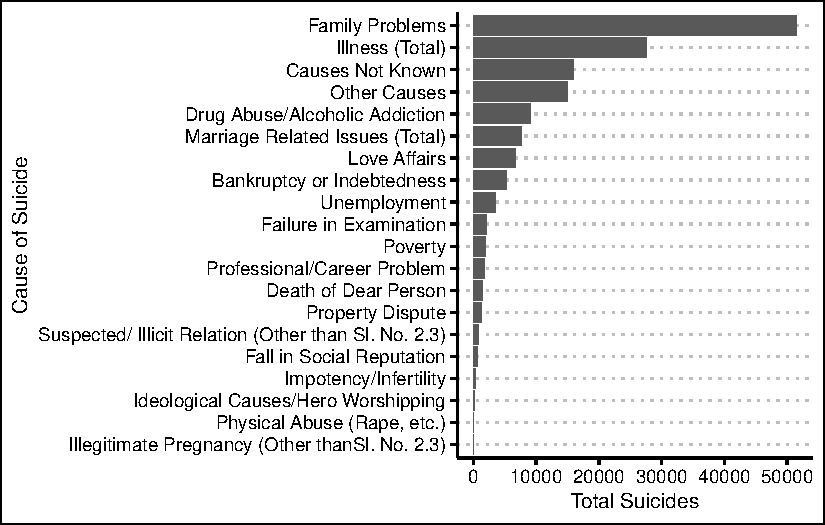
\includegraphics{file_files/figure-pdf/unnamed-chunk-7-1.pdf}

}

\end{figure}

You might want to visualize this separating by gender. For that, you
will need to ``tidy'' the data. One function that comes in handy for
this is \textbf{pivot\_longer()}. Then, I can use the gender (male,
female, transgender) to decide the colour fill. Like always, learn more
about the function by typing \textbf{?pivot\_longer()} in your console.

\begin{Shaded}
\begin{Highlighting}[]
\NormalTok{df }\SpecialCharTok{\%\textgreater{}\%} 
   \FunctionTok{select}\NormalTok{(cause, total\_male, total\_female, total\_transgender) }\SpecialCharTok{\%\textgreater{}\%} 
   \FunctionTok{pivot\_longer}\NormalTok{(}\SpecialCharTok{!}\NormalTok{cause, }\AttributeTok{names\_to =} \StringTok{"gender"}\NormalTok{, }\AttributeTok{values\_to =} \StringTok{"suicides"}\NormalTok{)}
\end{Highlighting}
\end{Shaded}

\begin{verbatim}
# A tibble: 60 x 3
   cause                           gender            suicides
   <chr>                           <chr>                <dbl>
 1 Bankruptcy or Indebtedness      total_male            4744
 2 Bankruptcy or Indebtedness      total_female           468
 3 Bankruptcy or Indebtedness      total_transgender        1
 4 Marriage Related Issues (Total) total_male            3484
 5 Marriage Related Issues (Total) total_female          4152
 6 Marriage Related Issues (Total) total_transgender        0
 7 Failure in Examination          total_male            1147
 8 Failure in Examination          total_female           933
 9 Failure in Examination          total_transgender        0
10 Impotency/Infertility           total_male             125
# ... with 50 more rows
\end{verbatim}

Now, let's plot this. You can learn more about this syntax at the
\href{https://r-graph-gallery.com/48-grouped-barplot-with-ggplot2.html}{R
Graph Gallery}. They have a fantastic collection of visualizations
possible with R and Python.

\begin{Shaded}
\begin{Highlighting}[]
\NormalTok{df }\SpecialCharTok{\%\textgreater{}\%} 
   \FunctionTok{select}\NormalTok{(cause, total\_male, total\_female, total\_transgender) }\SpecialCharTok{\%\textgreater{}\%} 
   \FunctionTok{pivot\_longer}\NormalTok{(}\SpecialCharTok{!}\NormalTok{cause, }\AttributeTok{names\_to =} \StringTok{"gender"}\NormalTok{, }\AttributeTok{values\_to =} \StringTok{"suicides"}\NormalTok{) }\SpecialCharTok{\%\textgreater{}\%} 
   \FunctionTok{ggplot}\NormalTok{(}\FunctionTok{aes}\NormalTok{(}\AttributeTok{x =} \FunctionTok{reorder}\NormalTok{(cause, suicides), }\AttributeTok{y =}\NormalTok{ suicides, }\AttributeTok{fill =}\NormalTok{ gender)) }\SpecialCharTok{+}
   \FunctionTok{geom\_col}\NormalTok{() }\SpecialCharTok{+}
   \FunctionTok{labs}\NormalTok{(}\AttributeTok{x =} \StringTok{"Cause of Suicide"}\NormalTok{, }\AttributeTok{y =} \StringTok{"Total Suicides"}\NormalTok{, }\AttributeTok{fill =} \StringTok{"Gender"}\NormalTok{) }\SpecialCharTok{+}
   \FunctionTok{scale\_fill\_discrete}\NormalTok{(}\AttributeTok{labels =} \FunctionTok{c}\NormalTok{(}\StringTok{"Female"}\NormalTok{, }\StringTok{"Male"}\NormalTok{, }\StringTok{"Transgender"}\NormalTok{)) }\SpecialCharTok{+}
   \FunctionTok{scale\_x\_discrete}\NormalTok{(}\AttributeTok{labels =}\NormalTok{ \textbackslash{}(x) }\FunctionTok{str\_wrap}\NormalTok{(x, }\AttributeTok{width =} \DecValTok{30}\NormalTok{)) }\SpecialCharTok{+}
   \FunctionTok{coord\_flip}\NormalTok{() }\SpecialCharTok{+}
\NormalTok{   ggthemes}\SpecialCharTok{::}\FunctionTok{theme\_clean}\NormalTok{(}\AttributeTok{base\_size =} \DecValTok{9}\NormalTok{) }\SpecialCharTok{+}
   \FunctionTok{theme}\NormalTok{(}\AttributeTok{legend.position =} \FunctionTok{c}\NormalTok{(}\FloatTok{0.8}\NormalTok{, }\FloatTok{0.2}\NormalTok{))}
\end{Highlighting}
\end{Shaded}

\begin{figure}[H]

{\centering 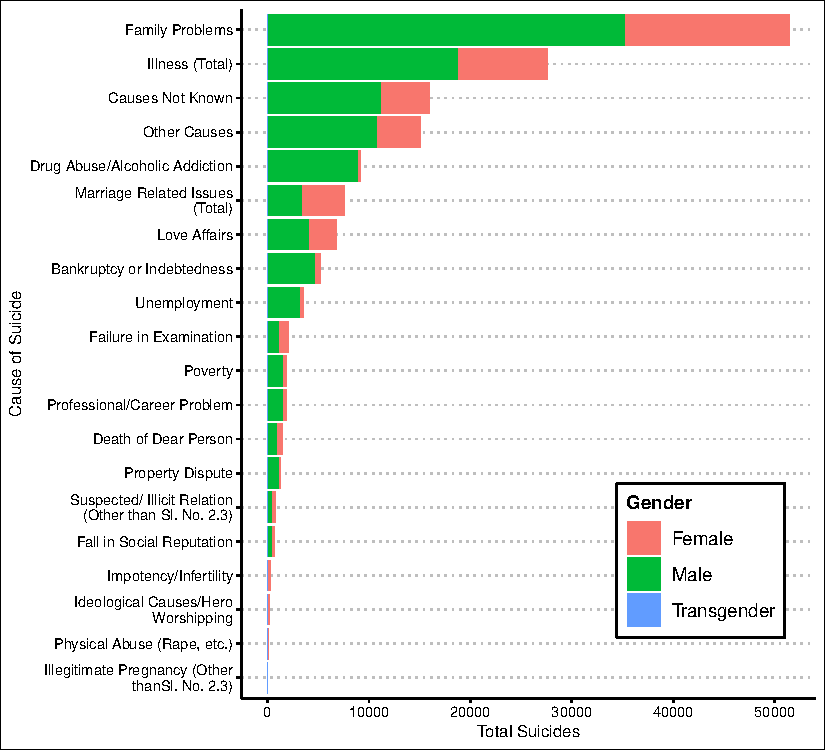
\includegraphics{file_files/figure-pdf/unnamed-chunk-9-1.pdf}

}

\end{figure}

The suicide rate is a lot higher for males than for females. The trend
is discernible in almost all categories. We can do all of this with just
a few lines of code. Intriguing, right?

\hypertarget{additional-resources}{%
\section{Additional Resources}\label{additional-resources}}

If you are looking for more resources around R, you should look at this
section.

\hypertarget{big-book-of-r}{%
\subsection{Big Book of R}\label{big-book-of-r}}

Big Book of R is a collection of mostly free and paid books about data
analysis and R. You can find books on virtually any topic.

\begin{itemize}
\item
  \href{https://www.bigbookofr.com/art.html}{aRtistry: Making Art with
  R}
\item
  \href{https://www.bigbookofr.com/data-science.html}{Data Science}
\item
  \href{https://www.bigbookofr.com/data-visualization.html}{Data
  Visualization}
\item
  \href{https://www.bigbookofr.com/machine-learning.html}{Machine
  Learning}
\item
  \href{https://www.bigbookofr.com/finance.html}{Finance}
\item
  \href{https://www.bigbookofr.com/geospatial.html}{Geospatial Data}
\item
  \href{https://www.bigbookofr.com/sport-analytics.html}{Sports
  Analytics}
\item
  \href{https://www.bigbookofr.com/time-series-analysis-and-forecasting.html}{Time-series
  Analysis}
\item
  and more.
\end{itemize}

\hypertarget{r-for-data-science-2nd-edition}{%
\subsection{R for Data Science, 2nd
Edition}\label{r-for-data-science-2nd-edition}}

It is the most popular book of R in the present world, with the web
version freely available. It talks about data wrangling, data
visualization, tidy principles, among other things. Hadley Wickham,
Chief Data Scientist at RStudio, is the leading author of the book. If
you want to dive into R deeply, this is where you should start. It is
available at \url{https://r4ds.hadley.nz}.

\hypertarget{next-today-i-learnt-about-r}{%
\subsection{Next --- Today I Learnt About
R}\label{next-today-i-learnt-about-r}}

Many of you have probably read and worked with R in the past. This
weekly newsletter, written by yours truly, presents byte-sized
information about R and data science. The format is pretty simple.
\textbf{There are five stories about the data world, four R packages,
three statistics and data science jargon, then two tweets about R and
one meme.} It is available for free. I promise, no spam.

https://www.getrevue.co/profile/harshbutjust

I might be biased, but this is probably the best way to remain updated
on new developments and come across interesting data science stuff. Here
are some past editions that I like.

\begin{itemize}
\item
  \href{https://www.getrevue.co/profile/harshbutjust/issues/is-r-squared-useless-next-issue-20-1053921}{Is
  R-squared Useless? \textbar{} Next --- Issue \#20}
\item
  \href{https://www.getrevue.co/profile/harshbutjust/issues/street-maps-free-apis-and-topic-modelling-next-issue-33-1194833}{Street
  maps, free APIs and Topic Modelling \textbar{} Next - Issue \#33}
\item
  \href{https://www.getrevue.co/profile/harshbutjust/issues/creating-music-with-r-next-issue-39-1256602}{Creating
  music with R \textbar{} Next - Issue \#39}
\item
  \href{https://www.getrevue.co/profile/harshbutjust/issues/moore-s-law-for-everything-next-issue-41-1305182}{Moore's
  Law for Everything \textbar{} Next - Issue \#41}
\item
  \href{https://www.getrevue.co/profile/harshbutjust/issues/books-on-data-science-next-issue-42-1314984}{Books
  on Data Science \textbar{} Next - Issue \#42}
\end{itemize}

\hypertarget{concluding-remarks}{%
\section{Concluding Remarks}\label{concluding-remarks}}

In this longish post, I rambled about my favourite programming language.
I talked about its history --- how AT\&T Labs developed a language that
became super popular because it was free to modify. Then, I introduced
the present-day mechanics of R World --- RStudio, Tidyverse and R
Markdown (Quarto). Then, I gave a short example of data wrangling and
visualization using data on suicides in India. Family reasons are the
cause of most suicides; males commit more suicides than women.

Finally, I added additional resources you should look for to learn more
about R. Big Book of R is a good collection of books on virtually every
topic in data science. Hadley Wickham's R for Data Science is an
excellent starting point. My newsletter can bring fresh content to your
inbox for free every Wednesday.

Happy R!

\hypertarget{about-the-author}{%
\section{About the Author}\label{about-the-author}}

Harshvardhan is a second-year PhD student of Business Analytics and
Statistics at the Haslam College of Business, University of Tennessee.
His research interests are in the application of machine learning and
applied statistics in the supply chain domain. He tinkers with R, reads
some blogs, and makes coffee in his free time. He invites you to his
digital garden at \url{https://www.harsh17.in}.



\end{document}
